\documentclass[tikz,border=4pt]{standalone}
\usepackage[T1]{fontenc}
\usepackage{lmodern}
\renewcommand{\familydefault}{\sfdefault}
\usetikzlibrary{shapes.geometric,positioning,arrows.meta,calc,fit,backgrounds,decorations.pathreplacing}
\tikzset{
  node distance=6mm,
  every node/.style={font=\footnotesize,align=center,execute at begin node={\hyphenpenalty=10000\relax}},
  base/.style={draw=gray!60,fill=gray!12,minimum height=7mm,inner sep=2pt},
  term/.style={base,rounded corners=3.5mm,text width=30mm},
  proc/.style={base,text width=32mm},
  err/.style={base,text width=30mm,fill=gray!22},
  io/.style={base,trapezium,trapezium left angle=72,trapezium right angle=108,trapezium stretches=true,text width=28mm},
  dec/.style={base,diamond,aspect=2.4,text width=27mm,inner sep=0pt},
  % predefined process: a call to another procedure
  sub/.style={proc,inner xsep=3mm,path picture={
    \draw[gray!60] ([xshift=1.5mm]path picture bounding box.north west)--([xshift=1.5mm]path picture bounding box.south west)
                   ([xshift=-1.5mm]path picture bounding box.north east)--([xshift=-1.5mm]path picture bounding box.south east);}},
  go/.style={-{Stealth[length=2mm]},draw=gray!55!black},
  lab/.style={font=\scriptsize,fill=white,inner sep=1pt},
  frame/.style={draw=gray!60,dashed,rounded corners=2mm,inner sep=3mm},
  % memory diagrams
  cell/.style={draw=gray!60,fill=gray!12,minimum height=7mm,inner sep=1pt,font=\scriptsize},
  hot/.style={cell,fill=gray!35},
  note/.style={font=\scriptsize,text=gray!30!black},
}

\begin{document}
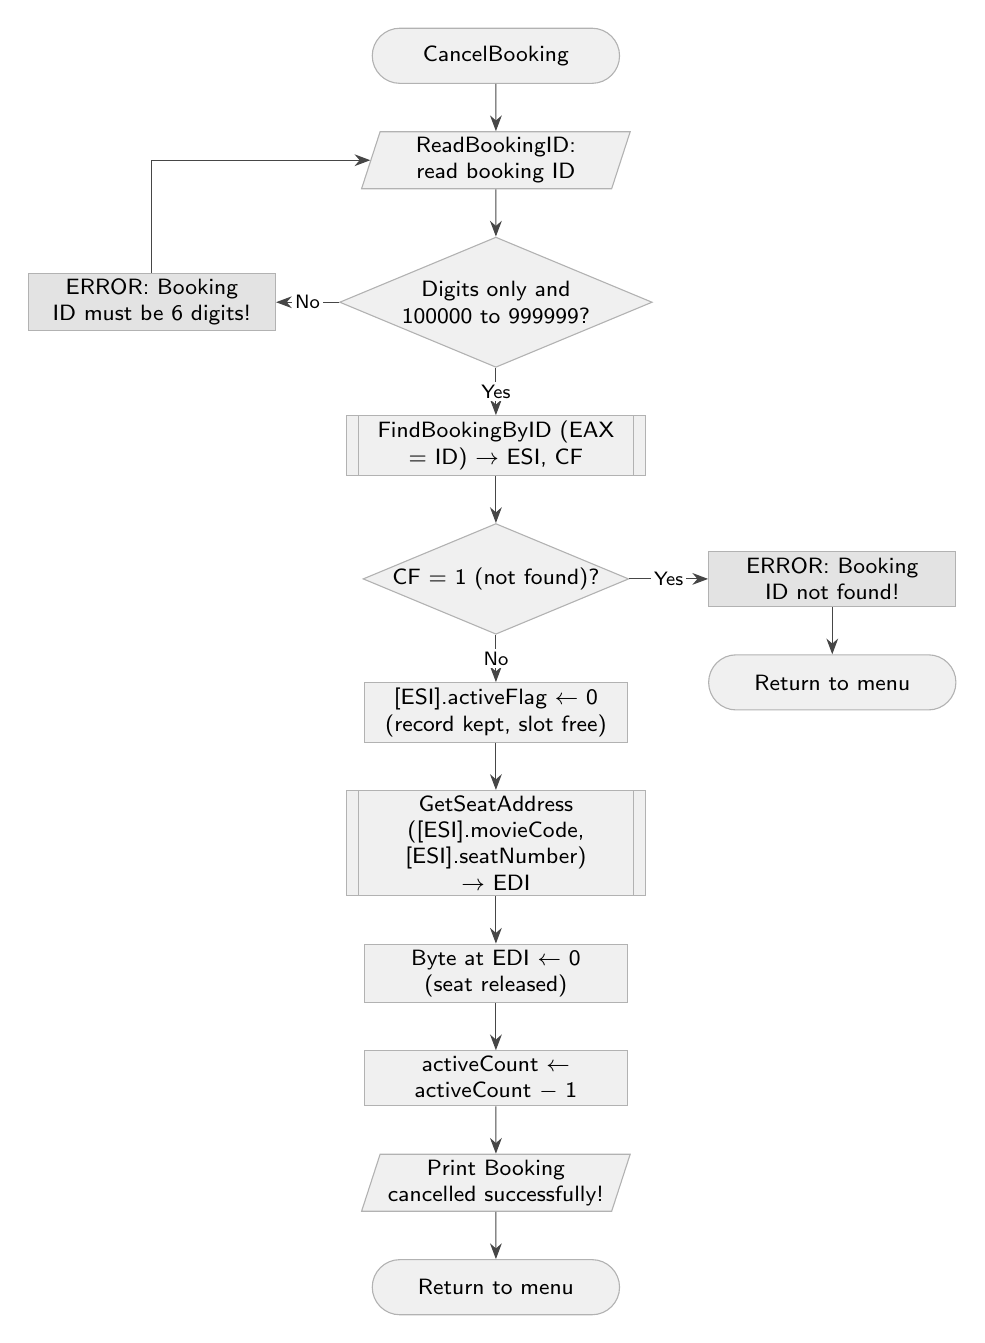
\begin{tikzpicture}
\node[term] (s) {CancelBooking};
\node[io,below=of s] (r) {ReadBookingID: read booking ID};
\node[dec,below=of r] (d1) {Digits only and 100000 to 999999?};
\node[err,left=8mm of d1] (e1) {ERROR: Booking ID must be 6 digits!};
\node[sub,below=of d1] (f) {FindBookingByID (EAX = ID) $\rightarrow$ ESI, CF};
\node[dec,below=of f] (d2) {CF = 1 (not found)?};
\node[err,right=10mm of d2] (e2) {ERROR: Booking ID not found!};
\node[term,below=of e2] (r2) {Return to menu};
\node[proc,below=of d2] (a) {[ESI].activeFlag $\leftarrow$ 0 (record kept, slot free)};
\node[sub,below=of a] (g) {GetSeatAddress ([ESI].movieCode, [ESI].seatNumber) $\rightarrow$ EDI};
\node[proc,below=of g] (z) {Byte at EDI $\leftarrow$ 0 (seat released)};
\node[proc,below=of z] (c) {activeCount $\leftarrow$ activeCount $-$ 1};
\node[io,below=of c] (ok) {Print Booking cancelled successfully!};
\node[term,below=of ok] (e) {Return to menu};
\draw[go] (s)--(r);
\draw[go] (r)--(d1);
\draw[go] (d1)--node[lab]{No}(e1);
\draw[go] (e1.north)|-(r.west);
\draw[go] (d1)--node[lab]{Yes}(f);
\draw[go] (f)--(d2);
\draw[go] (d2)--node[lab]{Yes}(e2);
\draw[go] (e2)--(r2);
\draw[go] (d2)--node[lab]{No}(a);
\foreach \a/\b in {a/g,g/z,z/c,c/ok,ok/e}{\draw[go] (\a)--(\b);}
\end{tikzpicture}
\end{document}
